%TODO
%TODO KC1) more general abstract - not necessarily just CMP
%TODO KC2) diagram of types of re-entry
%TODO KC3) include PVs in diagram
%TODO KC4) afterdepolarisation diagram
%TODO KC5) advantages of CA
%TODO TE1) check your words about rotor core slowdown make sense

% TODO source/sink stuff
% TODO fibres are reconstructions, which have same anisotropy but not much else
% TODO zhao - how was obtained
% TODO add start

\documentclass[a4paper, 12pt]{report}

\usepackage[a4paper, margin=2cm]{geometry}

% Optionals
\def\UrlBreaks{\do\/\do\-}
\usepackage[numbers]{natbib}

\usepackage{graphicx}
\usepackage{standalone}
\usepackage{float}
\usepackage{hyperref}
\usepackage{amsmath}
\usepackage{textcomp}
\usepackage{amssymb, gensymb}
\usepackage{bbm}
\usepackage{mathrsfs}
\usepackage{tabularx}
\usepackage{titlesec}
\usepackage{xspace}
\usepackage{subcaption}
\usepackage{tikz}
\usepackage{moreverb}
\usepackage{nameref}
\usepackage{csquotes}
\usepackage{mdframed}
\usepackage{tcolorbox}

\setcounter{tocdepth}{1}

\newcommand{\detailtexcount}[1]{%
  \immediate\write18{texcount -merge -sum #1.tex > #1.wcdetail }%
  \verbatiminput{#1.wcdetail}%
}

\newcommand{\texcount}[1]{%
  \immediate\write18{expr `texcount -merge -sum -total -brief #1.tex` > #1.wcsimple}%
  \input{#1.wcsimple}%
}

\newcommand{\etalcite}[2]{%
    {#2}~\textit{et~al.}~\cite{#1}%
}

\usetikzlibrary{shapes,arrows,decorations.pathreplacing,decorations.markings,positioning,arrows.meta}
\tikzstyle{decision} = [diamond, draw=black,thick, minimum width=4cm, minimum height=3cm, text centered, inner sep=0em]
\tikzstyle{block} = [rectangle, draw=black,thick, text width=5em, text centered, minimum height=4em]
\tikzstyle{line} = [draw=black,thick, -{Stealth}]

\titleformat{\chapter}[block]
	{\normalfont\Large\bfseries}{Chapter \thechapter:}{0.5em}{}
\titlespacing*{\chapter}{0pt}{0pt}{20pt}

\usepackage{fancyhdr}
\pagestyle{fancy}
\rhead{}
\lhead{\nouppercase{\leftmark}}
\setlength{\headheight}{15pt}

\numberwithin{equation}{chapter}
\numberwithin{figure}{chapter}

\graphicspath{{./graphics/}}

\def\cmp{{Christensen-Manani-Peters}\xspace}
\def\projectfilename{{ProjectReport-01055136-AF}}

% This somehow ignores headers.
%TC:macro \cite [ignore]
%TC:macro \section [ignore]
%TC:macro \chapter [ignore]
%TC:macro \subsection [ignore]
%TC:macro \subsubsection [ignore]

\begin{document}

% Don't count title page
%TC:ignore	
	\begin{titlepage}
        \includegraphics[width=70mm]{IMP_ML_1CS_4CP}	
\vspace*{8cm}

\begin{centering}

	{\Huge \scshape CMTH-Christensen-1b}
	\vspace*{1cm}

	{\Huge Complexity Science Approach to Atrial Fibrillation}
	\vspace*{6cm}
	
	{\Large
	\begin{tabular}{rl}
		{\Large Author CID:} & {01055136} \vspace*{0.1cm} \\
		{\Large Supervisor:} & Professor Kim Christensen \vspace*{0.1cm} \\
		{\Large Assessor:} & Dr. Tim Evans \vspace*{0.1cm} \\
		{\Large Submitted:} & April 29, 2019 \vspace*{0.1cm} \\ % TODO change this date?
		{\Large Wordcount:} & \texcount{\projectfilename} \vspace*{0.1cm} \\
	\end{tabular}
	}

\end{centering}

	\end{titlepage}
%TC:endignore


	\begin{abstract}
        \normalsize \input{ch0_abstract.tex}
	\end{abstract}

% Don't count contents page
%TC:ignore	
	\tableofcontents
%TC:endignore

	\chapter{Introduction} \label{ch:introduction}
	Atrial fibrillation (AF) is the most common heart rhythm disorder~\cite{narayan2012treatment}, and causes parts of the heart to spasm (or `fibrillate') instead of contracting effectively~\cite{nattel}. It affects predominantly the elderly~\cite{wasmer2017predisposing}. As of 2010 it affected 8.8 million people over the age of 50 in the EU, and this number is expected to double by 2050~\cite{krijthe2013projections}. AF causes a five-fold increase in stroke risk, is responsible for 25\% of strokes in people over the age of 80~\cite{wolf1991probability}, and the strokes caused by AF are more severe than strokes from other causes~\cite{miller2005cost}. The direct cost of AF to the NHS was \pounds 459~million in 2000~\cite{stewart2004cost}. 
Typically treatments take the form of surgical interventions, but as AF has poorly-understood mechanisms these surgical interventions have a high risk of complications and a low success rate~\cite{deshmukh2013hospital, cappato2005worldwide}.

The \cmp (CMP) model is a simple model of AF. It treats the heart as a two-dimensional discrete square lattice, where each site represents a heart cell. The state of each cell evolves over time, controlled by a set of simple rules which are based on the behaviour of real heart cells. These simple rules enable fibrillation to arise spontaneously~\cite{cmp}.
	
\section{Aims and Objectives}

In this work, we create a computational model of AF based on information about the cardiac muscle configuration (a `fibre map') of a real sheep heart, in which heart cells act based on the rules defined by the CMP model. Our specific aims are as follows:
\begin{enumerate}
    \item Demonstrate the feasibility of generalising the CMP model to a more realistic three-dimensional anatomy based on a sheep heart. We intend to move away from the lattice structure imposed by the CMP model, and towards a complex network structure possessing large-scale structural anisotropy reflective of a real sheep heart. We hope to verify that the core results of the original model are preserved in this generalisation.
    \item Determine the spatial distribution of electrical anomalies that drive AF and compare to the clinically measured distribution.
    \item Find computationally efficient ways to locate these electrical anomalies.
    \item Assess future clinical applications of this model, with a focus on whether this model can guide surgical interventions to improve their efficacy.
\end{enumerate}

\section{Related Works}

This project builds on or extends several related works:
\begin{itemize}
    \item \etalcite{cmp}{Christensen} defined the simple rules for cell behaviour that we adapt to a more complex geometry. 
    \item \etalcite{zhao}{Zhao} produced the fibre map from a sheep heart, which we are using to guide the creation of this geometry. They also designed a model of atrial fibrillation, but modelled the heart as a continuum in which electrical impulses are conducted with anisotropic propagation speeds. In comparison, our approach phenomenologically models individual cells.
    % \item The Master's thesis of Menkus~\cite{menkus} also built on this atrial fibre map but retained the discrete lattice structure of the CMP model; we discard this constraint, thereby solving several issues in the way electrical signals travel through the atrium.
\end{itemize}

\section{Report Outline}

The outline of the remainder of this report is as follows:
\begin{description}
    \item[Ch. \ref{ch:biologicalbackground}: \nameref{ch:biologicalbackground}] summarises the biology necessary to understand the rules behind the modelling process. It ends with a brief summary of some of the modelling approaches that have been used to study AF.
    \item[Ch. \ref{ch:cmpmodel}: \nameref{ch:cmpmodel}] describes the simple model of AF developed by \etalcite{cmp}{Christensen}. It also describes the extensions we have made to this simple model in preparation for our generalised model.
    \item[Ch. \ref{ch:generalisation}: \nameref{ch:generalisation}] details our work generalising the \cmp model to a more realistic substrate. Our procedure to create the substrate for our generalised model is explained and justified. The results shown by our model are shown and discussed, with a focus on whether they are consistent with AF in real hearts. This chapter represents the bulk of the novel work in this project.
    \item[Ch. \ref{ch:conclusion}: \nameref{ch:conclusion}] summarises our findings and discusses the clinical implications of our model. The limitations and future research potential for our model are considered.
\end{description}
	
	\chapter{Background} \label{ch:biologicalbackground}
    \section{Heart Structure and Function}

The heart comprises four chambers: the left atrium, right atrium, left ventricle, and right ventricle. Deoxygenated blood enters the right atrium from the body, and is then pumped from the right ventricle to the lungs. Oxygenated blood from the lungs enters the left atrium via the pulmonary veins, and is then pumped from the left ventricle to the rest of the body~\cite{Weinhaus2005}. A simplified diagram of the heart is shown in Fig.~\ref{fig:heartdiagram}.

The wall of the heart is divided into three layers: the epicardium (outer layer), myocardium (middle layer) and endocardium (inner layer). By volume, the cells in the myocardium are mostly cardiomyocytes, also called cardiac muscle cells~\cite{clayton}. Cardiomyocytes are coupled to each other at `gap junctions' and are mostly joined end-to-end forming long chains. These chains are surrounded by a network of collagen (a type of protein) which provides physical support and groups them into muscle fibres~\cite{funck1997regulation}. In a healthy heart, there are many transverse connections between the muscle fibres, but these can be lost due to fibrosis. Fibrosis is a disease characterised by excessive collagen forming an insulating layer between muscle fibres. Fibrosis increases as the heart ages~\cite{luke1991remodeling} and is strongly associated with AF, but the mechanism behind this is not precisely understood~\cite{de2011fibrosis}.

The pace of the heart (or `sinus rhythm') is set by the sinoatrial node. This is a cluster of `pacemaker' cells in the right atrium, which are the source of an electrical signal that is conducted through the cardiomyocytes and causes the muscle fibres to contract~\cite{irisawa1993cardiac}.

The atrioventricular node conducts this signal from the atria to the ventricles, delaying signals to allow the atria to pump blood into the ventricles before the ventricles contract~\cite{campbell1997biology}. Fibrillating ventricles are immediately life-threatening. Fortunately, the atrioventricular node possesses some filtering ability, ensuring that even when the atria are fibrillating the ventricles will still contract normally, albeit at a higher rate~\cite{nattel}.

\begin{figure}[H] \begin{mdframed}
	\centering
	\includegraphics[width=\linewidth,trim=0 0.5cm 0 0,clip]{heart_diagram_withpvs}
	\caption{Simplified structure of the heart, as viewed from the front. Relevant anatomical features are indicated. The pulmonary veins are particularly relevant for atrial fibrillation~\cite{haissaguerre1998spontaneous, ehrlich2003cellular}. Adapted from~\cite{gary2016bayes}.}
	\label{fig:heartdiagram}
\end{mdframed} \end{figure}

\subsection{Action Potential and Signal Propagation}

The membrane potential is the potential difference across the cell membrane of a cardiomyocyte, defined such that positive charge flowing into the cell makes it more positive~\cite{nattel}. The cardiac action potential is a rapid change in the membrane potential due to charges moving across gap junctions between cardiomyocytes. This action potential is what causes the cardiomyocytes to contract, giving rise to the sinus rhythm~\cite{katz2010physiology}. 
A typical cardiomyocyte action potential is shown in Fig.~\ref{fig:atrialcap}, with various phases indicated:
\begin{itemize}
	\item Phase 4 is the resting state of the cell. In this phase the cell can be excited by a neighbouring cell.
	\item Phase 0 is the depolarisation or excitation of the cell, caused by the membrane potential reaching a certain `threshold potential'. The membrane potential typically reaches this threshold because of a neighbouring cell also depolarising. In this way an electrical signal can propagate through the heart by exciting connected cardiomyocytes which in turn excite their neighbours.
	\item Phases 1--3 are the refractory period of the cell. During this stage it cannot be excited. This ensures that the signal cannot double back; that is, if cell A excites cell B, then cell B cannot immediately excite cell A in return. This behaviour gives rise to a mostly united wavefront for an electrical signal propagating through the atrium.
\end{itemize}

An electrocardiogram measures the electrical activity of the heart using electrodes on the skin~\cite{pullan2005mathematically}. This is an indirect measure of the electrical signals propagating through the heart due to the cardiomyocyte action potential.
%An intra-cardiac electrogram (henceforth referred to as an electrogram) is an ECG with several additional leads inserted into the heart. Both of these are indirect measures of the electrical signals propagating through the heart due to the action potential of the cardiomyocytes.

\begin{figure}[h!] \begin{mdframed}
	\centering
	\includegraphics[width=0.7\textwidth]{action_potential_frompathophys.jpg}	
	\caption{A typical ventricular cardiomyocyte action potential, with phases indicated. In phase 0 the cell is said to be `excited' or `depolarised'. Phases 1--3 are the refractory period of the cell, during which it does not respond to electrical signals. In phase 4 the cell is resting and excitable. The `membrane potential' is the potential difference across the cell membrane, and is defined such that it becomes more positive as positive charge enters the cell~\cite{nattel}. Adapted from~\cite{pathophys}.}
	\label{fig:atrialcap}
\end{mdframed} \end{figure}

\section{Atrial Fibrillation}

Atrial fibrillation is a heart rhythm disorder characterised by an elevated heart rate and ineffective contraction of the atria. It results from sources of electrical signals outside the sinoatrial node.
An episode of atrial fibrillation may be categorised by its length:
\begin{itemize}
    \item Paroxysmal if it self-terminates within 7 days.
    \item Persistent if it lasts longer than 7 days but less than 12 months.
    \item Long-standing persistent if it lasts more than 12 months.
    \item Permanent if physicians have ceased attempts to restore normal heart rhythm~\cite{uptodate}.
\end{itemize}

\subsection{Mechanisms}

The precise mechanisms of AF are unknown, but several competing theories exist.

\subsubsection{Focal Ectopic Sources} 

These are rapidly repeating spontaneous excitations of individual cardiomyocytes outside of the sinoatrial node (usually seen in the pulmonary veins~\cite{uptodate, haissaguerre1998spontaneous}). These are thought to result from problems in the electrochemistry of individual cells. If these excitations repeat fast enough, the cell will take over control of the heart rhythm and induce AF~\cite{nattel}.
This theory has fallen out of favour as the primary maintainer of AF. However, it is believed that focal ectopic sources can initiate AF, as studies have shown that spontaneous cardiomyocyte excitations in the pulmonary veins may trigger the arrhythmia~\cite{haissaguerre1998spontaneous}.
	
\subsubsection{Re-entry Circuits}

Re-entry circuits are self-sustaining looping signals.
An `anatomical' re-entry circuit arises when a signal reaches an anatomical obstacle, such as a region of fibrosis, as illustrated in Fig.~\ref{fig:litreviewreentry}.

\begin{figure} \begin{mdframed}
    \centering
    \begin{subfigure}[b]{0.8\textwidth}
        \includegraphics[width=\textwidth]{re_entry_formation_1}
        \caption{A signal enters from the cardiomyocyte on the left. It splits at the junction, and the signal on the upper branch continues while the signal on the lower branch is halted by some form of intermittent or unidirectional conduction block.  \\ }
    \end{subfigure}
    
    \begin{subfigure}[b]{0.8\textwidth}
        \includegraphics[width=\textwidth]{re_entry_formation_2}
        \caption{The signal continues to propagate on the upper branch, splitting at each junction it meets. \\ }
    \end{subfigure}
    
    \begin{subfigure}[b]{0.8\textwidth}
        \includegraphics[width=\textwidth]{re_entry_formation_3}
        \caption{The signal ends up back on the lower branch, and passes through the conduction block. From here the signal will keep looping indefinitely.}
    \end{subfigure}
    \caption{Formation of an anatomical re-entry circuit. Each pink box represents a cardiomyocyte. The black arrowheads represent the wavefront of a signal, while their tails represent the refractory cells left in the wake of the signal. The large gap in the middle is an example of an anatomical obstacle.}
    \label{fig:litreviewreentry}
\end{mdframed} \end{figure}

The `refractory tail' (the refractory cells left in the wake of a signal) means that there is a minimum size for a re-entry circuit. Any smaller and the signal will collide with its own refractory tail and be extinguished. This minimum length is called the `wavelength of re-entry', and is given by product of the refractory period and conduction velocity~\cite{rensma1988length}. This explains why studies have found that decreasing the refractory period increased the risk of AF~\cite{rensma1988length}.

Functional re-entry is a re-entry circuit that forms around a `functional obstacle' rather than an anatomical obstacle. The nature of this functional obstacle varies between theories. For example, in `leading circle theory', the circuit generates a signal that propagates towards the centre of the circuit (as well as outwards), meaning that the centre of the circuit is composed of refractory tissue; the centre of the circuit therefore acts as a functional obstacle. Clinical observations incompatible with leading circle theory (namely that certain pharmacological treatments can reduce incidence of AF despite reducing the wavelength of re-entry) mean that this hypothesis has fallen out of favour~\cite{calkins2007hrs}.
`Rotors' are another hypothesised type of functional re-entry. In rotors, the centre of the circuit cannot be excited due to the high curvature of the part of the wave near the core~\cite{waks2014mechanisms} which lowers the speed of conduction due to the way a cell distributes current to its neighbours; the core therefore acts as a functional obstacle. Some studies purport to have found rotors in real hearts~\cite{Narayan1761}, but this is disputed~\cite{calkins2007hrs}.

A proposed resolution to the apparent discrepancy between focal and re-entrant drivers is that focal sources are not the primary driver, and are only observed due to limited resolution in surface mapping, only mapping one side of the heart, and complications from the way that re-entrant sources inside the heart project onto the surfaces~\cite{hansen}. Further research is needed to confirm or reject this hypothesis.
	
\subsection{Remodelling} \label{subsec:remodelling}

AF modifies the heart over time to make it a more favourable substrate for AF~\cite{wijffels1995atrial}. For example, sustained AF appears to promote fibrosis~\cite{burstein2007atrial, CORRADI20141250}, which in turn promotes AF~\cite{de2011fibrosis}. Additionally, if a cell is excited at a very high rate it will shorten its refractory period%
%in order to avoid an excessively high concentration of certain ions
~\cite{gaspo1997functional}, shortening the wavelength of re-entry and allowing more re-entry circuits to form. Both of these processes are examples of remodelling. In many cases paroxysmal AF progresses to persistent AF; remodelling provides one explanation for this~\cite{deVos2010progression}.

\subsection{Treatment}

The first line of treatment for AF is usually antiarrhythmic drugs, some of which work by lengthening the refractory period of the cardiomyocytes~\cite{bajpai2006atrial}. These are often used in combination with anticoagulants, as blood clots that form in the atria during AF can cause strokes~\cite{bajpai2006atrial}. However, antiarrhythmic drugs are not without risk and can themselves cause life-threatening rhythm disorders~\cite{nattel1998experimental}. Additionally, when used in the absence of surgical treatments, they only have a success rate of 16\%~\cite{wilber2010comparison}.

If pharmacological treatments for AF are unsuccessful, catheter ablation is used instead. This means using a catheter, inserted into a vein and guided to the heart, to surgically destroy or isolate regions of tissue responsible for AF. However, locating these regions is a difficult challenge. It has been found that 52\% of patients undergoing ablation experience no further episodes of AF, and a further 24\% experience no further episodes when using antiarrhythmic drugs as well as ablation~\cite{cappato2005worldwide}. In addition to this poor success rate, 6\% of ablation procedures have complications~\cite{deshmukh2013hospital}, which is why it is typically used only after antiarrhythmic drugs have failed.

As the pulmonary veins are a common substrate for both ectopic sources~\cite{haissaguerre1998spontaneous} and re-entry circuits~\cite{ehrlich2003cellular}, pulmonary vein isolation is a common ablation procedure involving electrically isolating the pulmonary veins from the rest of the atrium~\cite{calkins2007hrs}. 

Various methods have been proposed for determining regions to ablate~\cite{narayan2012treatment, nademanee2004new, hunter2011characterization, kottkamp2016box, miller2014initial, sommer2016successful} but they are generally unreliable or have failed to be reproduced in subsequent studies~\cite{calkins2007hrs, BUCH2016636, verma2015approaches, providencia2015there}. 
% Examples include isolating areas of high fibrosis, ablating areas which appear to show multiple deflections of electrical signals, and ablating rotors directly.

% \subsection{Mapping AF Drivers}

% A complex fractionated atrial electrogram is an electrogram that indicates multiple deflections of a propagating signal lasting longer than a particular length of time. A 2004 study found that ablating in areas showing these electrograms was effective at curing AF~\cite{nademanee2004new}. Later studies have failed to reproduce this effect~\cite{verma2015approaches, providencia2015there}, but one study found that particular classifications of complex fractionated atrial electrograms were a good indication of areas to ablate~\cite{hunter2011characterization}. Further study may be required.

% There are other novel methods for determining regions to ablate. Isolation of areas with high fibrosis in combination with pulmonary vein isolation has shown promising initial results~\cite{kottkamp2016box}. Ablation of rotors  showed promising initial results~\cite{narayan2012treatment, miller2014initial, sommer2016successful} but other studies have failed to reproduce these~\cite{BUCH2016636}.

\section{Modelling Atrial Fibrillation}

Due to the difficulties of studying AF in living patients, it is desirable to design models instead. Models give greater control over the parameters of the atria than would be possible in an experimental setting, and are not invasive. Some models of cardiac electrophysiology model the heart as a continuum with anisotropic conduction properties; these are extremely fast to simulate, but may not reproduce phenomena arising from interactions between cells. Others consider the behaviour of ion currents between cells, but these are so computationally intensive that simulating even a single heartbeat is slow~\cite{Butters20120067, harrild2000computer, zhaoperformance}.

A middle ground between these two modelling approaches is to use cellular automata. In a cellular automaton, cells on a lattice are treated as discrete units with a finite number of states. At each step of the model, the new state of each cell is determined by its own state and the state of other cells in its neighbourhood~\cite{wolfram1983statistical}. Cellular automata don't take into account the full complexities of the internal behaviour of cells or detailed interactions between them, so may not reproduce phenomena emerging from these more detailed interactions. Additionally, a cellular automaton cannot model long-term changes or rate-dependent effects~\cite{pullan2005mathematically}, such as remodelling.
Despite these limitations, the cellular automaton approach carries significant advantages. The cardiomyocytes are discrete and, under this approach, they are treated as such. The simplified nature of this approach also allows the model to run extremely fast, so large quantities of data can be collected for analysis. Cellular automata can still be useful even if the internal workings of the cardiomyocytes are not well-understood or are extremely difficult to simulate, as this detail is abstracted away.

\section{Key Points from Chapter \thechapter}

\begin{itemize}
    \item Atrial fibrillation is caused by abnormal behaviour of electrical signals in the heart; anatomical re-entry circuits are especially important in the upcoming chapters.
    \item Treatments for AF are ineffective and attempts to locate re-entry circuits have historically been disappointing.
    \item Fibrosis results in fewer connections between muscle fibres, and has been implicated in AF.
    \item The heart cells obey an action potential with three distinct phases: excited $\rightarrow$ refractory $\rightarrow$ resting. This behaviour allows electrical signals to be conducted through the atrium.
    \item Cellular automata are a natural choice when modelling the heart, and carry enormous speed advantages compared to more detailed models.
\end{itemize}


		
	\chapter{The \cmp Model} \label{ch:cmpmodel}
	\section{Lattice and Algorithm} \label{sec:cmpalgo}

The \cmp (CMP) model is a cellular automaton which shows fibrillation-like behaviour. The myocardium is represented by a square lattice with side length $L$, and discrete sites, each representing a single cardiomyocyte. Sites can be coupled to their nearest neighbours, which means that they can interact; these couplings are analogous to the gap junctions in cardiomyocytes. Each site is coupled to its neighbours in the `longitudinal' direction (left-right in Fig.~\ref{fig:cmp}) 100\% of the time, whereas it is coupled to its neighbours in the `transverse' direction (up-down in Fig.~\ref{fig:cmp}) with some probability $\nu$. This reflects the structure of the myocardium, in which cells are arranged in long fibres which occasionally branch to form transverse connections~\cite{de2011fibrosis}. In the transverse direction, there are periodic boundary conditions, meaning that this lattice is really a thin cylindrical shell. This very loosely approximates the topology of a real atrium~\cite{cmp}.

 \begin{figure}[b!] \begin{mdframed}
 	\centering
 	\includegraphics[width=0.45\linewidth]{cmp}
 	\caption{Diagram of an example CMP model lattice with $L=3$. The black boxes represent cardiomyocytes and the couplings between them represent gap junctions between cardiomyocytes. The sites in the leftmost column are the pacemakers, which spontaneously excite at a regular rate. In the left-right direction, every possible nearest-neighbour coupling exists. In the up-down direction, nearest-neighbour couplings exist with probability $\nu$. This reflects the branching structure of the myocardium, which has long fibres with occasional transverse connections between them. The labels `transverse' and `longitudinal' are therefore a natural choice when labelling the two axes. Adapted from~\cite{cmp}.}
 	\label{fig:cmp}
 \end{mdframed} \end{figure}

Each site in the model has three possible states, updated at each timestep of the model based on their own state and that of their coupled neighbours. The allowed states (and their corresponding phases in the cardiac action potential shown in Fig.~\ref{fig:atrialcap}) are:
\begin{itemize}
    \item excited (phase 0)
    \item resting (phase 4)
    \item refractory (phases 1--3).
\end{itemize}
The sites on the leftmost edge of the lattice are defined to be `pacemaker' sites, analogous to the sinoatrial node in the atrium. Their states are set to excited each time a fixed number of timesteps has elapsed.
5\% of sites (chosen randomly) are designated `defective', meaning they have a 5\% chance of failing to excite when the model rules dictate they should~\cite{cmp}.

The rules determining the evolution of the state of each site are shown in flowchart form in Fig.~\ref{fig:cmpalgo}. Based on these simple rules, a propagating signal arises, analogous to the electrical signal that propagates through the atrium~\cite{cmp}.

Re-entry circuits can arise in the model when a defective site fails to excite. Figure~\ref{fig:cmpreentry} explains how a re-entry circuit might form, and why they form more often when $\nu$ is small. Note that this is the simplest example of a re-entry circuit; circuits found in the model can be far more complicated than the example shown and often multiple re-entry circuits may form at the same time.

In order to determine computationally whether the system is fibrillating, we tracked the number of times each site was excited. If the site with the highest number of excitations was a pacemaker, then the system was not fibrillating. Otherwise, we concluded that a site has been excited more times than the pacemakers and therefore must be part of a re-entry circuit. This metric was chosen because it generalises well to 3D and more complicated geometries. More obvious metrics like `number of sites excited at a given time greater than some threshold' only work in this very simple 2D model because it is homogeneous at large scales and so the number of excited cells changes little over a pacemaker period. However, it must be noted that this choice of metric introduces a source of error to the model: re-entry circuits are only detected after they complete their first loop, and their termination is only detected after the subsequent excitation of the pacemakers. When measuring the number of timesteps spent in AF, this introduces an error of up to approximately one pacemaker period per episode of AF. % TODO how negligible?

\begin{figure}
	\centering
    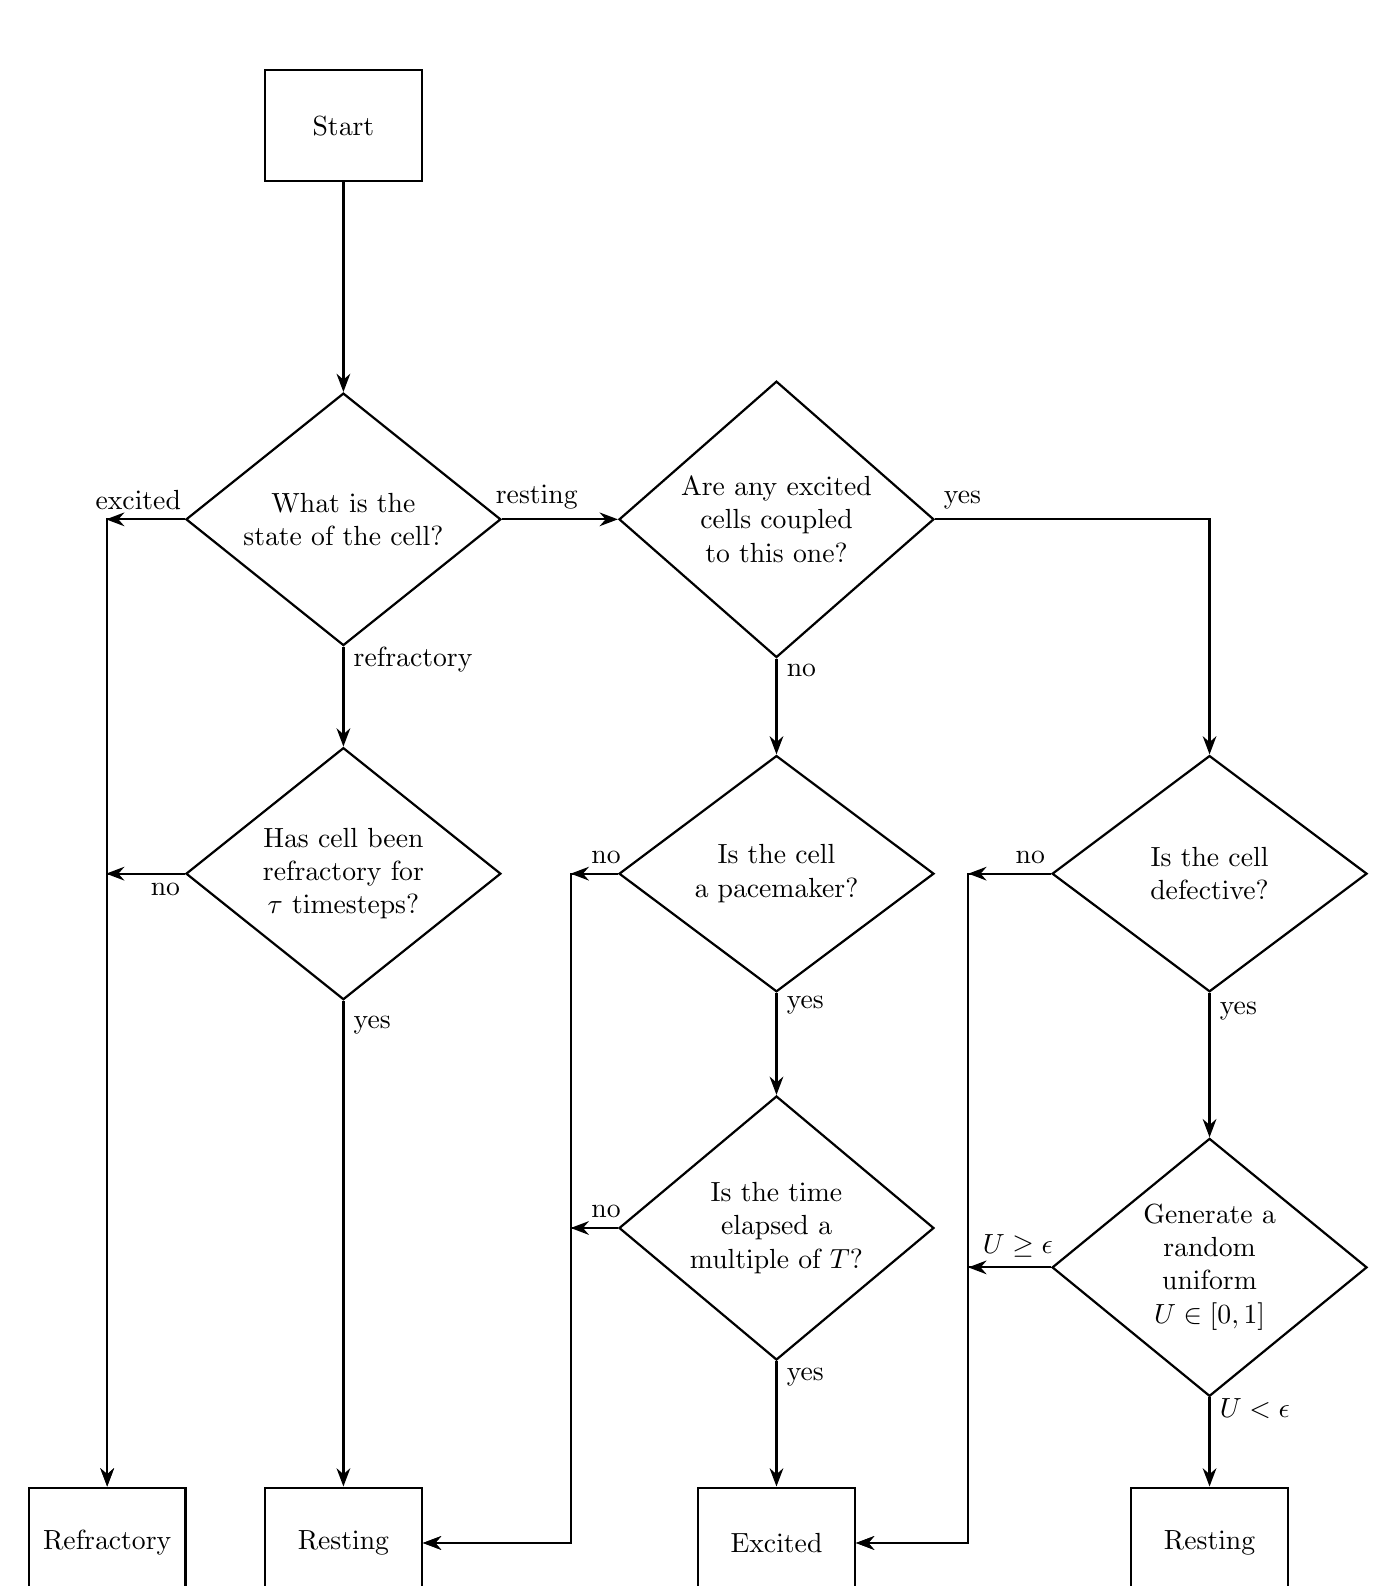
\begin{tikzpicture}[node distance=5cm,align=center,auto]
	\node[decision](start){What is the \\ state of the cell?};
    \node[block, above of=start](realstart){Start};
	\node[decision, below of=start, node distance=4.5cm](refractory){Has cell been \\ refractory for \\ $\tau$ timesteps?};
	\node[decision, right of=start, node distance=5.5cm](excited){Are any excited \\ cells coupled \\ to this one?};
	\node[decision, below of=excited, node distance=4.5cm](pacemaker){Is the cell \\ a pacemaker?};
	\node[decision, below of=pacemaker, node distance=4.5cm](pacemakerperiod){Is the time \\ elapsed a \\ multiple of $T$?};
	\node[decision, right of=pacemaker, node distance=5.5cm](defective){Is the cell \\ defective?};
	\node[decision, below of=defective](defectivecheck){Generate a \\ random \\ uniform \\ $U \in [0, 1]$};
	\node[block, below of=pacemakerperiod, node distance=4cm](excitedend){Excited};
	\node[block, left of=excitedend, node distance=5.5cm](restingend){Resting};
	\node[block, left of=restingend, node distance=3.0cm](refractoryend){Refractory};
	\node[block, right of=excitedend, node distance=5.5cm](restingend2){Resting};
	
	\path[line](realstart)       -- (start);
	\path[line](start)           -- node[very near start]{refractory} (refractory);
	\path[line](refractory)      -| node[very near start]{no}         (refractoryend);
	\path[line](refractory)      -- node[pos=0.05]{yes}        (restingend);
	\path[line](start)           -- node[pos=0.3]{resting}    (excited);
	\path[line](excited)         -- node[very near start]{no}         (pacemaker);
	\path[line](pacemaker)       -- node[very near start]{yes}        (pacemakerperiod);
	\path[line](pacemaker.west) -| node[above, very near start]{no} ++(-0.6, 0) |- (restingend);
	\path[line](excited)         -| node[pos=0.05]{yes}        (defective);
	\path[line](defective)       -- node[very near start]{yes}        (defectivecheck);
	\path[line](defective.west) -| node[above, very near start]{no} ++(-1.05, 0) |-         (excitedend);
	\path[line](defectivecheck)  -- node[very near start]{$U < \epsilon$}         (restingend2);
	\path[line](defectivecheck.west) -| node[above, pos=0.2]{$U \ge \epsilon$} ++(-1.05, 0) |- (excitedend);
	\path[line](pacemakerperiod) -- node[very near start]{yes}        (excitedend);		
	\path[line](pacemakerperiod.west) -| node[above, very near start]{no} ++(-0.6, 0) |- (restingend);
	\path[line](start)           -| node[above, pos=0.3]{excited}    (refractoryend);
	
	\path[line] (defective.west) -- ++(-1.05, 0);
	\path[line] (defectivecheck.west) -- ++(-1.05, 0);
	\path[line] (pacemaker.west) -- ++(-0.6, 0);
	\path[line] (pacemakerperiod.west) -- ++(-0.6, 0);
	\path[line] (refractory.west) -- ++(-1.00, 0);
	\path[line] (start.west) -- ++(-1.00, 0);
\end{tikzpicture}
    \caption{The algorithm used to determine the next state of the cell; this should be run for every cell in the lattice and the results should be stored before making any changes. Then, all state changes can be applied at once. $\tau$ is the refractory period of each heart cell, $T$ is the pacemaker period, and $\epsilon = 0.05$ is the probability of a defective cell failing to excite.}
    \label{fig:cmpalgo}
\end{figure}

\begin{figure} \begin{mdframed}
	\centering
	\includegraphics[width=0.7\linewidth]{cmp_reentry_2}
	\caption[short caption]{Diagram showing the formation of a simple re-entry circuit. A white square is an excited cell; a black square is a resting cell. Refractory cells start off light grey and progress to dark grey.
	At $t=0$, a signal is propagating along both the upper and lower branch. The red box indicates a defective cell, which fails to excite at $t=1$ thus extinguishing the signal along the lower branch, which is why at $t=3$ there is only conduction along the upper branch. At $t=7$, it can be seen that the signal has crossed over a transverse connection onto the lower branch. From here it is obvious that the signal can keep propagating in a loop until the defective cell fails again (which only happens with probability 5\%).
	Note that if the right transverse connection was too close to the left one, there would still be refractory cells on the lower branch by the time the wavefront looped back around, and the circuit would be extinguished. This is why there are no circuits for large $\nu$. This also explains why for small $\nu$ the fibrillation is persistent; in this regime, many re-entry circuits form so the chance of all of them being inactive at the same time is vanishingly small. 
	This large gap between transverse fibres is analogous to an anatomical obstacle, so re-entry circuits in the CMP model are anatomical rather than functional. Diagram adapted from~\cite{cmp}.}
	\label{fig:cmpreentry}
\end{mdframed} \end{figure}

\clearpage
\section{Results from Literature}


There is a threshold value of the connection fraction $\nu = \nu^*$. When $\nu \gg \nu^*$, no re-entry circuits form and the wave propagates longitudinally. When $\nu \ll \nu^*$, re-entry circuits form spontaneously and produce persistent fibrillation. When $\nu \approx \nu^*$, self-terminating or `paroxysmal' AF appears. In the real myocardium, the transverse connectivity is reduced by fibrosis, which has been implicated in atrial fibrillation~\cite{de2011fibrosis}. This result is therefore consistent with clinical observations. This dependence of atrial fibrillation risk on $\nu$ is summarised in Fig.~\ref{fig:cmpriskcurve}. It is possible to derive a theoretical form of this `risk curve' by neglecting boundary effects:
\begin{equation}
    P_\mathrm{risk} = 1 - (1 - (1 - \nu)^\tau)^{\delta L^2},
\end{equation}
where $P_\mathrm{risk}$ is the fraction of time fibrillating, $\tau$ is the refractory period (in simulation timesteps), $\delta$ is the fraction of cells which are defective, and $L$ is the side length of the square lattice. One can see that when $\nu \ll 1$, this value is approximately one. When $\nu$ gets larger, $(1 - \nu)^\tau$ quickly starts to decrease, causing $P_\mathrm{risk}$ to rapidly drop off towards zero. This theoretical form is also shown in Fig.~\ref{fig:cmpriskcurve}. Figure~\ref{fig:cmpreentry} explains why $\nu$ has this effect on re-entry circuits in the model.

Some further work on this model used machine learning to pinpoint re-entry circuits, given an electrocardiogram of the lattice. In tissue containing a single re-entry circuit, its location was correctly estimated in 95.4\% of cases~\cite{mcgillivray2018machine}. This suggests that with a more realistic fibre structure, this model could find clinical use for locating re-entry circuits.

\begin{figure}[h!] \begin{mdframed}
    \centering
    \includegraphics[width=0.66\textwidth]{cmp_risk_curve}
    \caption[short caption]{The CMP `risk curve', so-called because it shows how the risk of AF varies with $\nu$. When generating our data, 50 different lattices were generated at each point in a graph, and the fraction of time fibrillating was measured over $10^6$ timesteps in each. Hence each point on the graph is a mean over 50 runs, and the error bars are calculated using the standard error of the mean. The data from our implementation shows good agreement with the data from the original implementation by \etalcite{cmp}{Christensen}. The agreement with theory is reasonable, but there is some departure due to boundary effects, as these are neglected when deriving the theoretical form~\cite{manani}. 
    At small $\nu$, the atria are in persistent fibrillation. At high $\nu$ there is no fibrillation. There is a `transition region' in the middle where the heart spends a finite amount of time fibrillating, which we describe as `paroxysmal'. }
\label{fig:cmpriskcurve}
\end{mdframed} \end{figure}

\clearpage
\section{Methodology from Our CMP Implementation}

We implemented the CMP model from scratch to develop a proof-of-concept algorithm to find re-entry circuits, that we later generalised to a more realistic topology.

\subsection{Verification}

First, we verified that the model had been correctly implemented by reproducing the risk curve from the original CMP paper. In order to do this, we randomly generated $50$ lattices for each value of $\nu$ under consideration. Then, the model was run for $10^6$ timesteps for each lattice. The fraction of time spent fibrillating was recorded for each lattice, and mean fraction was plotted against $\nu$ in Fig.~\ref{fig:cmpriskcurve}. Our data showed good agreement with the risk curve data from the original CMP paper, confirming that the implementation of the algorithm was valid. There was some error in the measured fraction due to the time at the start of the simulation when the model had not yet had time to start fibrillating. This was mitigated by running for a number of timesteps that is much larger than the pacemaker period ($10^6 \gg T$).

\subsection{Locating Re-entry Circuits} \label{sec:locating}

We developed an algorithm that will eventually find the shortest re-entry circuit currently active in the model. We first ran the model until fibrillation arose. The algorithm, explained in Fig.~\ref{fig:reentryalgo}, builds a tree structure to locate looping signals. We defined it in a general way that doesn't depend on the structure of the CMP lattice, so it becomes easy to generalise to higher dimensions or more complicated geometries. It is intentionally iterative rather than recursive, which reduces the number of slow Python function calls.

\begin{figure} \begin{mdframed}
    \centering
    \begin{subfigure}[b]{0.46\textwidth}
        \includegraphics[width=\textwidth, trim={0cm 6cm 0 6cm}, clip]{tree_1}
        \caption{The algorithm starts by creating a tree with a single node (referred to as the `root node'), representing the cell that was first excited more times than the pacemakers. We define $t$ to be the time at which it becomes excited more times than the pacemakers. Therefore, at $t$ the re-entry circuit has just completed its first loop. Any node corresponding to this cell is labelled D. \\}
    \end{subfigure}
    ~
    \begin{subfigure}[b]{0.46\textwidth}
        \includegraphics[width=\textwidth, trim={0 6cm 0 6cm}, clip]{tree_2}
        \caption{Cells that are coupled to the start cell and are excited at time $t-1$ are added as children to the root node. In this exemplar case there are two such cells. The next step in the algorithm will be to consider the excited neighbours of these two cells at time $t - 2$, adding them as grandchildren to the root node. \\ \\}
    \end{subfigure}
    
    \begin{subfigure}[b]{0.92\textwidth}
        \includegraphics[width=\textwidth]{tree_3}
        \caption{This process is repeated until the original cell cell is added to the tree again. Once this happens we can trace a route (red) from the original cell at the bottom to the root node. The nodes lying on this route represent the cells in the circuit.}
    \end{subfigure}
    % \end{mdframed}
    \caption{Our algorithm used to locate re-entry circuits. It always finds the shortest re-entry circuit active in the model. It must be stressed that this is a highly simplified example; our real trees are much larger and more complicated.}
    \label{fig:reentryalgo}
\end{mdframed} \end{figure}

\subsection{Centrality Measurements} \label{sec:centrality}

The circuit-finding algorithm defined in Sec.~\ref{sec:locating} is computationally intensive, so a more computationally efficient proxy for re-entrant activity is desirable.
As previously established, for a re-entry circuit to form, transverse connections must be sufficiently far apart. This requires a fibre to be mostly isolated, which necessarily means cells on that fibre will have few connections. 

Centrality measures quantify how well-connected a particular site is, which means that cells on an isolated fibre would have low centrality. Many of these are extremely computationally intensive for large numbers of sites, or consider scales much greater than the size of a re-entry circuit.
However, a less computationally intensive option is harmonic centrality:
\begin{equation}
    H_i = \sum_{j \ne i}^N \frac{1}{d_{ij}}, \label{eq:harmonic}
\end{equation}
where $i$ is the index of the cell for which we want to calculate centrality, $N=40,000$ is the number of cells, and $d_{ij}$ is the minimum number of connections that have to be traversed in order to reach cell $i$ from cell $j$. We expected this to be useful because unlike many other centrality measurements, it weights the local area around cell $i$ very highly. One can see that cells on an isolated stretch of fibre are going to have a much lower value of $H_i$ than those on a well-connected stretch, as the shortest path to most other sites will have to go through a long stretch of isolated fibre. Thus we would expect low centrality to indicate high re-entrant activity.

The time required to calculate $H_i$ for $N$ sites would scale as $\sim N^2$. However, since the CMP model is homogeneous on large scales, one does not need to actually sum all the way up to $N$ to calculate $H_i$; instead one can sum over all sites with $d_{ij} < D$, where $D$ is some threshold distance greater than the length of a typical isolated stretch. The terms that are neglected average out to a `background' contribution that is approximately the same at any point in the lattice. This turns a problem that is quadratic in $N$ into a problem with more favourable complexity. Preliminary tests found that there was no noticeable difference between $D=20$ and $D\rightarrow\infty$, so we chose $D=20$ as our cutoff.

\section{Results from Our CMP Implementation}

For illustrative purposes, a plot showing re-entry circuits next to reciprocal centrality measurements (i.e. $1 / H_i$) is shown in Fig.~\ref{fig:centralitycomparison}; there appears to be some correlation but it is difficult to ascertain how strong this correlation is. Figure~\ref{fig:cvcall} shows how well centrality predicts re-entrant activity. We found that low centrality is a good predictor of re-entrant activity, and that low centrality is a much better predictor at values of $\nu$ within the transition region than outside. Low centrality is a worse predictor at very small $\nu$ because re-entry circuits can form almost anywhere and centrality is low almost everywhere.

\begin{figure}[h!] \begin{mdframed}
    \centering
    \begin{subfigure}[b]{0.46\textwidth}
        \includegraphics[width=\textwidth]{circuit_map_binary}
        \caption{The locations of the re-entry circuits found for a particular lattice. Most of the circuits are long and narrow like the example in Fig.~\ref{fig:cmpreentry}, so in this visualisation (in which there are no gaps between adjacent cells) they look like bars.}
    \end{subfigure}
    ~
    \begin{subfigure}[b]{0.46\textwidth}
        \includegraphics[width=\textwidth]{centrality_harmonic_reciprocal}
        \caption{The centrality measurements for the cells on the lattice. We have shown the reciprocal because low centrality is associated with re-entry circuits. The centrality is lower at the left and right edges because those cells have fewer neighbours.}
    \end{subfigure}
    \caption{Side by side comparison of re-entrant activity and centrality measurements for a particular lattice with $\nu = 0.14$. Ignoring the edge-effects in (b), there is correlation. Axis units are integer grid coordinates rather than real distance measurements.}
\label{fig:centralitycomparison}
\end{mdframed} \end{figure}

\begin{figure}
    \begin{mdframed}
    \centering
    \includegraphics{circuits_v_centrality_harmonic_ALL}
    \caption{How well does centrality predict re-entry? Inside the transition region at $\nu=0.15$, a cell with very low centrality has a 26\% chance of hosting a re-entry circuit, but outside the transition region centrality is a worse predictor. The spike at high centrality is likely because high-centrality cells have many pathways going through them, so re-entry circuits happen to pass through them as a matter of chance. Though the data is binomial (as each cell either has a circuit or not), there are many points in each bin so a Gaussian approximation was used to calculate the standard error of the mean for the error bars.}
    \label{fig:cvcall}
\end{mdframed} \end{figure}

\clearpage
\section{Implementation} \label{sec:cmpimpl}

We implemented the CMP model ourselves in C++, providing a Python interface through the Python/C~API. This has all the performance advantages of C++, while allowing NumPy for data analysis and Matplotlib for producing high-quality visualisations. This fast, flexible implementation would not be feasible using either language in isolation.

We implemented from scratch all the code required to run this model, find re-entry circuits, and measure centrality. This required 1722 lines of Python code and 1512 lines of C++ code, with 81 lines in miscellaneous build scripts. The total number of lines of code was 3315. We used no external libraries other than the standard Python libraries, Matplotlib, and NumPy.

We used several techniques to improve performance, besides improvements to algorithmic complexity already mentioned. Finely tuning the compiler with the aid of profiling tools allowed for powerful optimisations in performance critical areas of the code; with this information we found seemingly trivial changes like reversing loop orders and replacing modulo operations with if-statements saw speed increases of around 10\% each. When calculating statistics we leveraged multiprocessing in order to spread the workload across several CPU cores at once. Instead of applying the algorithm described in Fig.~\ref{fig:cmpalgo} to every cell, we kept track of excited cells and only considered the cells bordering them; this produced identical behaviour whilst having to loop over fewer cells. We used bitmasks (binary numbers where the individual bits represent booleans such as presence of connections or whether a cell is defective) to store properties of each cell as this gave significant performance gains and saved on memory. We avoided using nested structures such as vectors of vectors, preferring to flatten these lists to make use of CPU caching.

\section{Key Points from Chapter \thechapter}

\begin{itemize}
    \item The CMP model is a cellular automaton that obeys simple rules, summarised in Fig.~\ref{fig:cmpalgo}. These rules are based on the behaviour of real heart cells.
    \item We define the model to be fibrillating when any non-pacemaker cell has been excited more times than the pacemakers.
    \item The CMP model has a control parameter $\nu$ which is analogous to fibrosis in the real heart, and affects risk of AF.
    \item We have designed an algorithm to find re-entry circuits that is easily generalised to higher dimensions and more complex geometries.
    \item Low harmonic centrality is a good predictor of re-entrant activity.
\end{itemize}

	
	\chapter{Generalisation to a Sheep Atrium} \label{ch:generalisation}
	The CMP model treats the heart as homogeneous on large scales with a constant fibre orientation, and assumes that the heart is shaped like a cylindrical shell. This means it cannot reproduce phenomena that are dependent on large-scale heterogeneity or specific anatomical features, which severely limits its clinical applications. Our novel generalisation of the CMP model to include both large-scale heterogeneity and anatomical features is therefore an important extension to the model.

% This particular 

\section{Sheep Heart Data}

We were provided with a sheep atrium fibre map by \etalcite{zhao}{Zhao}
in the form of a discrete 3-dimensional vector field. At each point in this vector field, there is a direction vector that represents the prevailing muscle fibre direction in a $50~\mathrm{\mu m} \times 50~\mathrm{\mu m} \times 50~\mathrm{\mu m}$ cube (or `voxel') centred on that point. If the direction vector for a particular voxel is the zero vector, there is no atrial muscle in that voxel. The magnitude of the direction vector has no biological relevance (unless it is zero), so we normalised the non-zero direction vectors before proceeding.


\section{Model Preparation}

To convert the sheep heart fibre map to a usable format, we applied fibre tracking algorithms to reconstruct the muscle fibres of the heart, giving a network embedded in 3D space.
Generating the network is a multi-step, computationally intensive process. The final procedure is outlined in the following subsections, and the choices made are justified at the end of this section. A small section of one such network is shown in Fig.~\ref{fig:sample}, for illustrative purposes.

It should be noted that the network we produced was not the same as the original sheep heart; the fibre map does not contain sufficient information to do this~\cite{jiang2006dtistudio}. However, our network reproduces the anisotropy of the network and includes key anatomical features like the pulmonary veins.

\begin{figure} \begin{mdframed}
    \centering
    \includegraphics[width=0.7\textwidth]{sample}
    \caption{A small section of a finished network. Each point is a site that obeys the rules of the CMP model, and each line between sites represents a connection. In this example the fibres mostly lie along the x-axis.}
    \label{fig:sample}
\end{mdframed} \end{figure}

\subsection{Coarse Graining}

In order to make the network generation computationally feasible, the vector field was first coarse-grained. For a coarse graining factor of $g$, this meant taking the sum of all vectors in each separate $g \times g \times g$ cube in the original vector field, then normalising the new vector to have unit length. This reduced each linear dimension by a factor of $g$ and the total volume by $g^3$. We took $g = 6$ in order to attain the computational speed necessary for good statistics, whilst retaining as much anatomical detail as possible.

When we change the model dimensions in this way, we are decreasing the length scale of the model by a factor of $g$. However, the real time required for a signal to cross the atrium must remain the same, so we have to decrease the time scale of the model by a factor of $g$ (thus reducing the refractory period and pacemaker period). This means that the conduction velocity is unchanged by coarse graining.

\subsection{Fibre Tracking}

We have chosen to adapt the Fibre Assignment by Continuous Tracking (henceforth called `FACT') algorithm, which was developed for reproducing networks of the brain from MRI data and is well-established in the field of neuroscience~\cite{fact, bello2008motor}. The algorithm produces a fibre given a vector field, and works as follows~\cite{fact}:
\begin{enumerate}
    \item Pick a point to be a `seed point'. We used the centre of each non-empty voxel.
    \item Find the direction of the vector field in the voxel containing that seed point, and then follow this vector field until reaching the boundary of this voxel with another voxel. Store the coordinates of this intersection.
    \item Find the direction vector in this other voxel and then follow that until reaching a boundary with another voxel. Store the coordinates of this intersection. Keep repeating this process until one of the following termination conditions is met:
    \begin{enumerate}
        \item An empty voxel is reached (i.e. a voxel where the direction vector is zero).
        \item The fibre encounters a sharp turn, i.e. a turn where the angle between previous direction of the fibre and the new direction of the fibre is greater than $\sim 40 \degree$.
        \item The fibre reaches a certain length. We chose a length of $8~\mathrm{mm}$, as this is approximately the length of fibres in the human heart~\cite{schwinger1994failing}. Obviously there will be differences between a sheep heart and a human heart but it is likely that these lengths are similar enough for our purposes to provide an approximate estimate.
    \end{enumerate}
\end{enumerate}
For each seed point, we first followed the vector field forwards, then we followed it backwards. Our maximum-length termination condition was applied to both halves of the fibre separately, so the maximum length of a fibre in our model was actually $2 \times 8~\mathrm{mm}$. This is still acceptable because $8~\mathrm{mm}$ was only an approximate estimate. This gave us a list of points that defined a fibre. A simplified 2D version of this process is detailed in Fig.~\ref{fig:fact}.

We repeated the above process for every single non-empty voxel, giving a huge number of fibres. However, this resulted in two problems:
\begin{itemize}
    \item The fibres had unevenly spaced points because the fibre was defined by the list of intersections with voxel boundaries (see Fig. \ref{fig:fact}). The rules of the CMP model dictate that a signal can cross one connection between sites in one timestep. This meant that the conduction velocity was slower when points were close together and faster when they were far apart. We needed fibres to conduct at a uniform speed along their entire length.
    \item For each non-empty voxel in the vector field, we had a fibre. This led to a density of fibres that is both non-uniform and far higher than what is seen in the real heart.
\end{itemize}

\begin{figure} \begin{mdframed}
    \centering
    \includegraphics[width=0.7\textwidth]{fact}
    \caption{Behaviour of FACT algorithm in 2D. The black arrows indicate the vector field (i.e. the prevailing directions of the fibres). The large red dot is the starting position of the fibre tracing. From there, the vector field is traced both forwards and backwards. The tracing follows the field in a straight line until it reaches a boundary, and then it follows the new direction until it reaches the next boundary, and so on. We store all the intersections of the fibres with the voxel boundaries, and these define a fibre.
    The fibre is terminated when it reaches an empty square (lower left) or a sharp turn (upper right).}
    \label{fig:fact}
\end{mdframed} \end{figure}

\subsection{Interpolation}

To solve the problem of uneven conduction velocity, we interpolated along the fibres and placed points at equal distances along the fibre. To do this, we used the following algorithm:
\begin{enumerate}
    \item Let the position of the $i$th point along the fibre (counting from $i=0$ at one end of the fibre) be the vector $\mathbf{F_i}$.
    \item Calculate the cumulative distance along the fibre at each point. Let the $i$th cumulative distance be $C_i$. We define $C_0 = 0$, so for example $C_1 = \left| \mathbf{F_1} - \mathbf{F_0} \right|$ and $C_2 = C_1 + \left| \mathbf{F_2} - \mathbf{F_1} \right|$.
    \item To place a point a distance $x$ along the fibre, find the largest $C_i$ that is less than $x$, and note its index $i$. This was done using a binary search as the list of cumulative lengths is sorted by definition. This reduces the search time for a fibre with $N$ points from $\sim N$ (for a naive linear search) to $\sim \log(N)$; a significant improvement, especially for large fibres.
    \item Compute the vector: \begin{equation}
        \mathbf{F_i} + \frac{\mathbf{F_{i + 1}} - \mathbf{F_i}}{ \left| \mathbf{F_{i + 1}} - \mathbf{F_i} \right|} (x - C_i).
    \end{equation}
    This is the position of the point a distance $x$ along the fibre.
\end{enumerate}
For every fibre, we calculated a set of interpolated points with separation of 1 unit, corresponding to a real physical length of $g \times 50~\mathrm{\mu m}$. This ensured that points along the fibre were regularly spaced, thus solving the issue of irregular conduction velocity along fibres.

\subsection{Fibre Density Regulation}

To solve the problem of the fibre density being too high, we adapted the Spherical-deconvolution Informed Filtering of Tractograms (henceforth SIFT) algorithm, also well-established within the field of neuroscience~\cite{sift, stampfli2019subtle}. Since we don't have the information about how the actual fibre density varies throughout the heart, we have assumed that the density is uniform.

Our adapted SIFT algorithm involves minimising a cost function $c$:
\begin{equation}
    c = \frac{1}{L} \sum_{\mathrm{voxels}} (l_v - \Bar{l}),
\end{equation}
where $L$ is the total length of all fibres, $l_v$ is the total fibre length in a specific voxel $v$, and $\Bar{l}$ is the target length per voxel. 

To minimise this function, we calculated the change to the cost function $\Delta c$ if each fibre were deleted. Then, we picked the fibre that has the highest $\Delta c / l_f$, where $l_f$ is the total length of the fibre. Long fibres go through many voxels and therefore will reduce the cost function more than short fibres; considering $\Delta c / l_f$ rather than $\Delta c$ ensured that the algorithm was not biased towards removing long fibres~\cite{sift}. This process was repeated, removing fibres until the cost function reached a target value. Once this was done, we had a set of fibres with roughly uniform density.

\subsection{Transverse Connectivity}

Finally, we can add `transverse' connections between nodes in adjacent fibres. To do this, we define a connection probability function. This is a sigmoid function, which can be thought of as a smoothed-out step function:
\begin{equation}
    p_\text{conn}(r) = \frac{1}{e^{b(r - \mu)} + 1},
    \label{eq:pconn}
\end{equation}
where $r$ is the distance between nodes, $b$ is the steepness of the transition region, and $\mu$ is a characteristic distance that controls where the centre of the step is. We chose $b = 7$ as it caused $p_\text{conn}$ to drop off quickly enough with $r$ that it rarely connected non-adjacent fibres.
This functional form is acceptable as it is $1$ for small $r$ but rapidly drops to $0$ once $r > \mu$.
A plot of $p_\text{conn}(r)$ is shown in Fig.~\ref{fig:pconn}.

\begin{figure}[h] \begin{mdframed}
    \centering
    \includegraphics[width=0.7\textwidth]{pconn}
    \caption{The connection probability function for $\mu=1$, plotted as a function of distance between nodes $r$. The function rapidly declines after reaching $r > \mu$. Units are defined such that the voxel side length is unity.}
    \label{fig:pconn}
\end{mdframed} \end{figure}

Calculating $p_\text{conn}$ for every pair of points would cause the time for completion (assuming $N$ nodes in the model) to scale with $N^2$, which is unacceptably slow for large $N$. To improve this, we stored a list of the nodes in each voxel. Then, when adding connections between nodes, we could consider the set of nodes in only nearby voxels without having to compute $r$ for every pair of nodes. This brings the time required to be approximately linear in $N$.

$\mu$ is analogous to the parameter $\nu$ in the original CMP model; by varying it, the connectivity between fibres changes. This means decreasing $\mu$ is also analogous to increasing fibrosis. The presence of this parameter makes it possible to reproduce the results of the original CMP model using our generalised model.

Note that by repeating this process of adding transverse connections but changing the initial state of the pseudorandom number generator, different networks could be generated for a single $\mu$ value. This enabled collection of better statistics.

\subsection{Justification}

\subsubsection*{Oblique Conduction Velocity}

We have made the deliberate choice to avoid aligning our nodes to a Cartesian grid.
This approach has benefits over a naive 3D generalisation of the CMP model in which nodes are aligned to a cubic lattice, because it allows for uniform conduction velocity along the fibres, regardless of the fibre direction. Figure~\ref{fig:staircase} illustrates how the naive approach leads to the problem of different conduction velocities in the oblique and cardinal directions. 

% Our approach also allows faithful reconstruction of the anisotropy of the sheep atrium, which can be only loosely approximated by the naive approach. This is because on a grid there are only a few possible directions that connect adjacent nodes.

\begin{figure}[H] \begin{mdframed}
    \centering
    \begin{subfigure}[b]{0.46\textwidth}
        \includegraphics[width=\textwidth]{staircase_oblique}
        \caption{$45\degree$ connections allowed}
    \end{subfigure}
    ~
    \begin{subfigure}[b]{0.46\textwidth}
        \includegraphics[width=\textwidth]{staircase_cardinal}
        \caption{$45\degree$ connections forbidden}
    \end{subfigure}
    \caption{The rules of the CMP model dictate that a signal crosses a connection (red) between two cells (black dots) in one timestep. In the cardinal directions we will therefore see a conduction velocity of one grid unit per timestep. However, in oblique directions the conduction velocity varies, which presents a problem: rotating the coordinate system would change the dynamics. This problem is illustrated under two possible rulesets for adding connections: in (a) $45\degree$ connections are allowed, and the conduction velocity in the oblique $45\degree$ direction is $\sqrt{2}$ grid units per timestep. In (b) we forbid oblique connections and the conduction velocity in the oblique direction is $\sqrt{2} / 2$ grid units per timestep. Neither of these are the same as the conduction velocity in the cardinal directions.}
    \label{fig:staircase}
\end{mdframed} \end{figure}

\subsubsection*{Why FACT and SIFT?}

This process was not the only one we tried; many weeks were required to settle on this process. The first process we tried was as follows:
\begin{enumerate}
    \item Pick an empty voxel (i.e. a voxel through which there are no fibres) and use as a seed point for FACT; fibres terminate if they enter a non-empty voxel, as well as if any of the previous termination conditions are met.
    \item Repeat for every empty voxel.
\end{enumerate}
However, this gave rise to unacceptable density variations depending on the orientation of the vector field, for reasons explained by Fig.~\ref{fig:firstattempt}. Variations in density will cause there to be more transverse connections in one place than another, which affects re-entry circuit formation and biases re-entry circuits to certain locations. Efforts to adapt $p_\text{conn}$ to correct for this bias were unsuccessful, so this approach had to be abandoned.

\begin{figure}[h] \begin{mdframed}
    \centering
    \includegraphics{firstattempt}
    \caption{An example of how our first attempt at producing a set of fibres from the atrial map can go wrong. Notice how the upper blue arrow (representing a potential transverse connection) is much shorter than the lower one. This happened because of a change in fibre direction, which is clearly unreasonable; the heart should not become more muscular in areas where the fibres are not aligned with the axes. Note that the left fibre has been terminated because it entered the same voxel as the right fibre.}
    \label{fig:firstattempt}
\end{mdframed} \end{figure}

We would expect the number of connections a node has to be approximately equal regardless of the direction of the fibre it lies upon. Figure~\ref{fig:angulardep} shows how the number of connections varies as a function of the angle between the fibre direction and the x-y plane, for both the FACT/SIFT approach, and this simpler approach.

\begin{figure}[h] \begin{mdframed}
    \centering
    \begin{subfigure}[b]{0.8\textwidth}
        \includegraphics[width=\textwidth]{angular_connectivity_original}
        \caption{Our first attempt}
    \end{subfigure}
    
    \begin{subfigure}[b]{0.8\textwidth}
        \includegraphics[width=\textwidth]{angular_connectivity_factsift}
        \caption{FACT/SIFT procedure}
    \end{subfigure}
    \caption{The connectivity of nodes as a function of fibre orientation. It can be seen that the FACT/SIFT approach gives a much more uniform connectivity (and therefore fibre density). The first attempt clearly shows that at oblique angles, the connectivity becomes lower, implying that the fibre density is also lower. The error bars (red) are the standard error of the mean. The drop for an angle of zero appears to be an artefact of the fibre map, as it appears under all our fibre tracking approaches.}
    \label{fig:angulardep}
\end{mdframed} \end{figure}

The main drawback to the FACT/SIFT approach is that the SIFT algorithm is extremely computationally intensive. Each time a fibre is removed, the quantity $\Delta c$ must be recalculated for every fibre, which scales with the number of fibres multiplied by the length of each fibre. However, SIFT is still faster than competing algorithms and avoids many of the same biases~\cite{sift}.

\clearpage
\section{Cell Behaviour}

The behaviour of individual cells is identical to the behaviour in the CMP model (summarised in Fig.~\ref{fig:cmpalgo}); we designated the same fraction (5\%) of cells defective, and they failed at the same rate (5\%). However, the pacemaker cells are now a small cluster in the right atrium, in the position of the sinoatrial node in the real heart. We designate any cells within a radius of 5 (corresponding to a distance of $5g \times 50~\mathrm{\mu m}$) of this point as pacemakers.
% TODO fill out the region

Note that in this generalised model, re-entry circuits form around anatomical obstacles in the same way as in the CMP model (previously explained in Fig.~\ref{fig:cmpreentry}). However, they can be significantly longer and more complicated. An example re-entry circuit from this generalised model is shown in Fig.~\ref{fig:newreentry}.

\begin{figure}[H] \begin{mdframed}
    \centering
    \includegraphics[width=1.0\textwidth]{circuit_example}
    \caption{An example of a re-entry circuit from the sheep atrium model, highlighted in red. The circuit has formed around a large empty region, which constitutes an anatomical obstacle. Note that this shows only a small subsection of the network. Axis units are in voxel coordinates.}
    \label{fig:newreentry}
\end{mdframed} \end{figure}

\clearpage 
\section{Results and Discussion}

This section presents the results of the generalised model. All results shown in this section are based on 1,000 different networks for each value of $\mu$, unless otherwise stated. Coarse graining of $g=6$ is used throughout.

\subsection{Risk Curve}

A necessary verification of this model is to produce a risk curve (first shown for the 2D CMP model in Fig.~\ref{fig:cmpriskcurve}). Obviously we can no longer vary the transverse connection fraction $\nu$, but we can instead vary $\mu$ (defined in Eq.~\eqref{eq:pconn}). At each value $\mu$ under consideration, the model was run for $10^5$ timesteps and the fraction of time for which it was fibrillating was recorded; this was repeated 100 times for each value of $\mu$. Note that the same definition of fibrillation used in our implementation of the CMP model was adopted for this model. The resulting risk curve is shown in Fig.~\ref{fig:ourriskcurve}. The risk curve is the shape we expect and shows both persistent and paroxysmal AF.
\begin{figure}[h] \begin{mdframed}
    \centering
    \includegraphics{risk_curve_3}
    \caption{The risk curve for the generalised model. Above $\mu \approx 1.25$, there is no fibrillation because the network is so well-connected that re-entry circuits are `shorted out'. Below $\mu \approx 1.00$ there is no fibrillation because there is no propagation at all; the signal dies out a short distance from the sinoatrial node. Note that each point represents the mean fraction of time in fibrillation for 1000 networks. Error bars are calculated using the $3 \times$ the standard error of the mean of the fractional time spent in AF, otherwise they would not be visible.}
    \label{fig:ourriskcurve}
\end{mdframed} \end{figure}

\clearpage

\subsection{Conduction Anisotropy}

The conduction velocity along fibres should be greater than the conduction velocity perpendicular to the fibres. In order to test this, an isotropic (or `null') model was created. The procedure to do this was as follows:
\begin{enumerate}
    \item Create an empty region containing no cells, of the same size as the region containing the original (`anisotropic') model.
    \item For every voxel in the original map that contains a cell, add a cell to this new model. This ensures that the null model has the same shape as the original.
    \item Add connections between these cells as a function of distance between them using Eq.~\eqref{eq:pconn}.
\end{enumerate}
This is enough to create a model that lacks the overall anisotropy of the sheep heart model, but otherwise looks very similar. We would expect the way the signal propagates through this model to be qualitatively different to the way it propagates through the real model. The result of running the model and measuring the time at which each cell is first activated is shown in Fig.~\ref{fig:activationtimes}. We see that we get the qualitative difference we expect.
Note that Fig.~\ref{fig:activationtimes} is derived from only a single network of the 1,000.

\begin{figure}[h] \begin{mdframed}
    \centering
    \includegraphics{activation_times_smooth}
    \caption{Time at which each cell in the model is first activated. This is a view of a quasi-two-dimensional slice through the heart. It can be seen that the activation patterns are qualitatively different, differing most noticeably in when the signal reaches the left atrium. We also see that the anisotropic model is much smoother, with fewer patches that are activated much later than their neighbours than in the isotropic case. The slight differences in shape of the two atria are caused by artefacts of the way the visualisation is generated and are not biologically relevant.}
    \label{fig:activationtimes}
\end{mdframed} \end{figure}

\clearpage

\subsection{Re-entry Circuit Distribution}

Our algorithm to find re-entry circuits in the original CMP model (see Fig.~\ref{fig:reentryalgo}) was used to find re-entry circuits in the sheep heart model. We designed this algorithm to work on a general network, so adapting it to this more complex substrate was a straightforward task. The spatial distribution of re-entry circuits in our model is shown in Fig.~\ref{fig:af_heatmap}.

It can be seen that the re-entry circuits mostly cluster around the sleeves of the pulmonary veins, with some re-entrant activity on the left atrial appendage and posterior left atrium; this is consistent with clinical observations~\cite{ehrlich2003cellular}. With increased fibrosis (corresponding to lower $\mu$) the area at risk of re-entrant activity increases, and correspondingly the risk of AF increases. This could explain why ablation strategies are less effective in persistent atrial fibrillation; if increased fibrosis results in more persistent fibrillation, and also increases the number of risk areas, the chance of destroying all re-entry circuits with an ablation becomes less favourable.

Most importantly, this highlights areas that have been implicated in drivers of AF by clinical studies, suggesting that regions of AF are in part caused by the fibre orientation in the atrium.

\begin{figure} \begin{mdframed}
    \begin{subfigure}[b]{0.92\textwidth}
        \centering
        \includegraphics[width=\textwidth]{{af_heatmap_mu=1.15_redo}.png}
        \caption{$\mu=1.15$}
    \end{subfigure}

    \begin{subfigure}[b]{0.92\textwidth}
        \centering
        \includegraphics[width=\textwidth]{{af_heatmap_mu=1.1_redo}.png}
        \caption{$\mu=1.1$}
    \end{subfigure}
    \caption{The probability of re-entry circuits over the surface of the atrium. Anything with a risk under 25\% is shown in grey for contrast. There is an increased risk of re-entry circuits on the sleeves of the pulmonary veins, especially the right superior pulmonary vein (RSPV on diagram), the left atrial appendage (LAA) and the posterior left atrium (PLA). It can be seen that as $\mu$ decreases, the risk regions increase in size and number, spreading to the right atrial appendage (RAA) and across the surface.}
    \label{fig:af_heatmap}
\end{mdframed} \end{figure}

\clearpage

\subsection{Harmonic Centrality}

The circuit finding algorithm was computationally intensive so a proxy was sought. The process applied here was almost identical to the process described in Sec.~\ref{sec:centrality}; re-entry circuits form in the same way as before so we would expect harmonic centrality to predict them effectively. When calculating $H_i$ we neglected summation terms where $d_{ij}$ was larger than 20. The calculated centrality was compared with the distribution of re-entry circuits. The results are shown in Fig.~\ref{fig:newcentrality}.

Centrality is a poor predictor of re-entrant activity in this model, which means that we have failed to find a computationally inexpensive proxy for re-entry. This may be because re-entry circuits in this model are much more complicated so they do not involve stretches of isolated fibre as they did in the CMP model. Additionally, large-scale heterogeneity makes the approximation used when calculating $H_i$ less valid than it was for the CMP model.

\begin{figure}[h] \begin{mdframed}
    \centering
    \includegraphics{circuits_vs_centrality_3}
    \caption{$H_i$ plotted against the probability of a circuit. It can be seen that harmonic centrality is no longer a useful predictor of re-entrant activity. Though the data is binomial (as each cell either has a circuit or not), there are many points in each bin so a Gaussian approximation was used to calculate the standard error of the mean for the error bars.}
    \label{fig:newcentrality}
\end{mdframed} \end{figure}

\clearpage


\section{Implementation}

As before, the model was written in C++ and Python using the Python/C API for the high-performance of C++ and the flexibility and libraries of Python. 

We were able to make use of Imperial's high performance computing cluster, allowing us to simulate 1000 networks per value of $\mu$. In order to achieve compatibility with Imperial's high performance computing facilities, much of the C++ had to be rewritten to an older standard. However, to simply run the model for a single heart, consumer hardware was more than sufficient.

We implemented from scratch every algorithm listed in this section, as well as the model itself. This required 6304 lines of code in total, with 3851 being C++ code required to run the simulation and another 2425 lines of Python code for data analysis or visualisation. We used no external libraries other than the standard Python libraries, Matplotlib, and NumPy.

We used several techniques to improve performance, besides improvements to the algorithmic complexity already mentioned. We duplicated many of the improvements discussed for the CMP model (Sec.~\ref{sec:cmpimpl}), such as profiling, and applying the cell update algorithm to only excited cells and their neighbours. 
% The model was implemented as a set of node objects which stored their state information and kept pointers to their neighbours, which meant that propagating signals through the model was much faster than implementations using other common ways to store networks.

\section{Key Points from Chapter \thechapter}

\begin{itemize}
    \item We have developed a procedure to turn a vector field representing the fibre orientation in a sheep atrium into a network model of the heart, where cells are not tied to a lattice. This procedure is computationally intensive but reduces density bias more than any other procedure we devised.
    \item We have a control parameter $\mu$ which is analogous to fibrosis in the real heart, and analogous to the control parameter $\nu$ from the CMP model. We find that the risk of atrial fibrillation varies in the expected way when we vary $\mu$, providing a necessary verification of the model's correctness.
    \item Our isotropic and anisotropic conduction models show qualitatively different behaviour, as expected and as shown in other models~\cite{zhao}.
    \item Harmonic centrality fails to predict re-entry on this generalised model.
    \item We find that the distribution of re-entry circuits in our model has good agreement with the clinically measured distribution, and that decreasing $\mu$ results in a larger risk area.
\end{itemize}


	\chapter{Conclusions} \label{ch:conclusion}
	We have successfully adapted the work of \etalcite{cmp}{Christensen} to a more realistic topology provided by \etalcite{zhao}{Zhao}. We found that our adaptation reproduces the core features of the CMP model, such as the dependence of AF risk on fibrosis with differences that can be explained by the changed structure. We found that our model shows anisotropy of conduction velocities and is qualitatively different from an isotropic null model. We also found that our model successfully identifies regions such as the pulmonary veins where clinical observations suggest are common substrates for re-entry circuits.

This is an important step towards developing the \cmp model into a useful tool that, with further work, may be possible to use in a clinical setting. We hope to present a summary of our work and results in the Computing in Cardiology 2019 conference.


\section{Limitations and Further Work}

This work is based only on a single sheep heart, so it is possible that other sheep hearts or human hearts would not reproduce these results. An obvious piece of further study would be to reproduce our results using a different fibre map.
We have also assumed uniform fibre density, conduction velocity, and fibrosis. However this is not reflective of the real heart~\cite{alonso2016nonlinear} and a fibre map that included this data would therefore be of interest.

Previous work with the CMP model has found that applying machine learning to an electrocardiogram (commonly called an ECG) can pinpoint a re-entry circuit with high accuracy~\cite{mcgillivray2018machine}. If this work were adapted to this more realistic geometry, it would be one step closer to being applicable in a clinical setting.

Centrality was effective on the CMP model, but not on the more realistic geometry. However, in this model re-entry circuits form around gaps in the fibre map (representing anatomical obstacles), so searching directly for gaps might prove a useful way to work out where re-entry circuits could form in a given fibre map.

At the coarse-graining levels used to gather statistics for the model ($g=6$), a voxel is $300~\mathrm{\mu m} \times 300~\mathrm{\mu m} \times 300~\mathrm{\mu m}$. The resolution of MRI when mapping heart fibres is approximately $1000 - 3000~\mathrm{\mu m}$ in clinical settings~\cite{mori2006principles} due to the motion of the heart. This means that our model is untested at a coarse-graining that is clinically attainable, so we can't conclude whether the model could be personalised for each patient. However, if further study concludes that these results hold at a lower resolution then personalised ablation patterns could be determined in mere minutes using consumer-grade hardware.


%TC:ignore
\clearpage
\section*{Acknowledgements}

Thank you to Dr. Nick Peters, Dr. Kishan Manani and Prof. Kim Christensen for developing the original \cmp model. Especially thank you to Prof. Christensen for supervising and guiding this project. Thank you to Max Falkenberg for support and feedback, and helping us write a manuscript to submit to a conference. Thank you to Alberto Ciacci for support and feedback. Thank you to Jichao Zhao for providing the fibre map. Thank you to Dr. Tim Evans for his comments and feedback. Thank you to my friends and family for their time spent providing feedback on this report. And a special thank you to my project partner for being a true collaborator and always having a relevant paper at the ready.

% \section*{Code Listings}

% All code can be 
%TC:endignore

% Don't count anything after references
%TC:ignore		
	\chapter{References} \label{ch:regerences}
	\bibliographystyle{naturemag}
	\renewcommand{\chapter}[2]{}
	\bibliography{bibliography}
	
% 	\detailtexcount{\projectfilename}
%TC:endignore
	
\end{document}
